\documentclass[14pt,aspectratio=169]{beamer}
\setbeamertemplate{caption}[numbered]
\setbeamertemplate{caption label separator}{:}
\setbeamercolor{caption name}{fg=normal text.fg}
\usepackage{amssymb,amsmath}
\usepackage{ifxetex,ifluatex}
\usepackage{fixltx2e} % provides \textsubscript
\usepackage{lmodern}
\ifxetex
  \usepackage{fontspec,xltxtra,xunicode}
  \defaultfontfeatures{Mapping=tex-text,Scale=MatchLowercase}
  \newcommand{\euro}{€}
\else
  \ifluatex
    \usepackage{fontspec}
    \defaultfontfeatures{Mapping=tex-text,Scale=MatchLowercase}
    \newcommand{\euro}{€}
  \else
    \usepackage[T1]{fontenc}
    \usepackage[utf8]{inputenc}
      \fi
\fi
% use upquote if available, for straight quotes in verbatim environments
\IfFileExists{upquote.sty}{\usepackage{upquote}}{}
% use microtype if available
\IfFileExists{microtype.sty}{\usepackage{microtype}}{}
\PassOptionsToPackage{hyphens}{url}
\usepackage{hyperref}
\usepackage{ulem}

% Comment these out if you don't want a slide with just the
% part/section/subsection/subsubsection title:
\AtBeginPart{
  \let\insertpartnumber\relax
  \let\partname\relax
  \frame{\partpage}
}
\AtBeginSection{
  \let\insertsectionnumber\relax
  \let\sectionname\relax
  \begin{frame}[plain]
    \tableofcontents[currentsection]
  \end{frame}
}
\AtBeginSubsection{
  \let\insertsubsectionnumber\relax
  \let\subsectionname\relax
  \frame{\subsectionpage}
}

\setlength{\parindent}{0pt}
\setlength{\parskip}{6pt plus 2pt minus 1pt}
\setlength{\emergencystretch}{3em}  % prevent overfull lines
\setcounter{secnumdepth}{0}
% Thanks Richard Darst on how to get a nice Beamer theme.
% See http://rkd.zgib.net/wiki/DebianBeamerThemes

\usepackage{multicol}
\usepackage[absolute,overlay]{textpos}
\usepackage{tikz}
\usepackage{ctable}
\usetikzlibrary{positioning}

\usebackgroundtemplate{
\includegraphics[width=\paperwidth]{images/swirl-lightest.pdf}}
\newif\ifplacelogo
\placelogotrue
\logo{\ifplacelogo
\includegraphics[viewport=274 335 360 440,width=1cm]{images/openlogo-nd.pdf}\fi}

\definecolor{debianred}{rgb}{.780,.000,.211} % 199,0,54
\definecolor{debianblue}{rgb}{0,.208,.780} % 0,53,199
\definecolor{debianlightbackgroundblue}{rgb}{.941,.941,.957} % 240,240,244
\definecolor{debianbackgroundblue}{rgb}{.776,.784,.878} % 198,200,224

\usetheme{Boadilla}
\setbeamertemplate{navigation symbols}{}

\usecolortheme[named=debianbackgroundblue]{structure}
\setbeamercolor{normal text}{fg=black}
\setbeamercolor{titlelike}{fg=debianblue}
\setbeamercolor{sidebar}{fg=debianred,bg=debianbackgroundblue}

\setbeamercolor{palette sidebar primary}{fg=debianred}
\setbeamercolor{palette sidebar secondary}{fg=debianred}
\setbeamercolor{palette sidebar tertiary}{fg=debianred}
\setbeamercolor{palette sidebar quaternary}{fg=debianred}

\setbeamercolor{section in toc}{fg=debianred}
\setbeamercolor{subsection in toc}{parent=debianred}

\setbeamercolor{item}{fg=debianred}

\setbeamercolor{block title}{fg=debianblue}


\title[Reproducible Builds tomorrow]{Reproducible
builds \\ where do we want to be tomorrow}
\subtitle{We've made lots of progress, \\
but we are still far from our goals \\
of changing the (software) world.}
\author[h01ger]{%
   \texorpdfstring{
            \centering
            Holger 'h01ger' Levsen
   }{h01ger}}
\date[All Systems Go!]{%
 All Systems Go! in Berlin, Germany\\
 \small{2017-10-21}}

\begin{document}
\placelogofalse

\begin{frame}[plain]
 \titlepage
\end{frame}

\placelogotrue

\begin{frame}
 \frametitle{about h01ger}

 \begin{itemize}
  \item \small{\texttt{B8BF 5413 7B09 D35C F026  FE9D 091A B856 069A AA1C}}
  \item Debian user since 1995, contributor since 2001, official developer
  status since 2007
  \item DebConf organizer,
  founded the DebConf video team
   \begin{itemize}
    \item \texttt{http://video.debian.net}
   \end{itemize}
 \item Debian-Edu (Debian for education)
  \item Debian QA (quality assurance)
  \begin{itemize}
   \item \texttt{https://piuparts.debian.org}
   \item \texttt{https://jenkins.debian.net} (~1200 jobs continously testing Debian)
  \end{itemize}
  \item Debian Reproducible builds team member
  \begin{itemize}
   \item since April 2015 funded by the Linux Foundation
   \item currently until December 2017…
 \end{itemize}
 \end{itemize}
\end{frame}

\begin{frame}
 \frametitle{Debian reproducible builds contributors}
 \begin{center}
  \begin{columns}
   \footnotesize
   \column{.30\linewidth}
    {akira} \\
    {Alexis Bienvenüe} \\
    {Andrew Ayer} \\
    {Asheesh Laroia} \\
    Boyuan Yang \\
    {Ceridwen} \\
    {Chris Lamb} \\
    {Chris West} \\
    {Christoph Berg} \\
    Clint Adams \\
    Dafydd Harries \\
    {Daniel Kahn Gillmor} \\
    {Daniel Shahaf} \\
    Daniel Stender \\
    David Suarez \\
    {Dhole} \\
    Drew Fisher \\
    Emmanuel Bourg \\
    Emanuel Bronshtein \\
    \column{.30\linewidth}
    Esa Peuha \\
    {Fabian Wolff} \\
    {Guillem Jover} \\
    Hans-Christoph Steiner \\
    Harlan Lieberman-Berg \\
    {Helmut Grohne} \\
    \only<1>{Holger Levsen}\only<2>{{\color{debianred} Holger Levsen}} \\
    HW42 \\
    Intrigeri \\
    {Jelmer Vernooij} \\
    {josch} \\
    Juan Picca \\
    Juliana Rodrigues \\
    {Lunar} \\
    Maria Glukhova \\
    Mathieu Bridon \\
    {Mattia Rizzolo} \\
    Nicolas Boulenguez \\
    {Niels Thykier} \\
    Niko Tyni \\
   \column{.30\linewidth}
    {Paul Wise} \\
    Peter De Wachter \\
    Philip Rinn \\
    {Reiner Herrmann} \\
    Robbie Harwood \\
    {Santiago Vila} \\
    {Sascha Steinbiss} \\
    {Satyam Zode} \\
    {Scarlett Clark} \\
    {Stefano Rivera} \\
    {Stéphane Glondu} \\
    {Steven Chamberlain} \\
    Tom Fitzhenry \\
    Vagrant Cascadian
    {Valerie Young} \\
    Valentin Lorentz \\
    {Wookey} \\
    {Ximin Luo} \\
  \end{columns}
 \end{center}
\end{frame}


\placelogofalse

\begin{frame}
 \frametitle{Who are you?}
 \begin{itemize}
  \item<2-4> Seen a talk about reproducible builds?
  \item<3-4> Contributed to these efforts?
  \item<4> Used reproducible builds as a user?
 \end{itemize}
\end{frame}

\begin{frame}
 \frametitle{Who are you?}
 \begin{itemize}
  \item Seen a talk about reproducible builds?
  \item Contributed to these efforts?
  \item Has verified locally running software (but which was built elsewhere) to actually be reproducible? IOW: Did a rebuild and got the exact same bits?
 \end{itemize}
\end{frame}



\section{Motivation}

\begin{frame}[fragile]
 \frametitle{The problem: we need to believe}
 \begin{itemize}
  \item Free Software is great: one can study, modify, share and use it!
  \item<2-4> We study, modify and share source code.
  \item<2-4> We use binaries.
  \item<3-4> We need to believe our binaries come from the source code they are said to made from.
  \item<4> \textbf{I don't want to believe.}
 
 \end{itemize}
\end{frame}

\begin{frame}
 \frametitle{The problem in greater detail}

 \begin{center}
  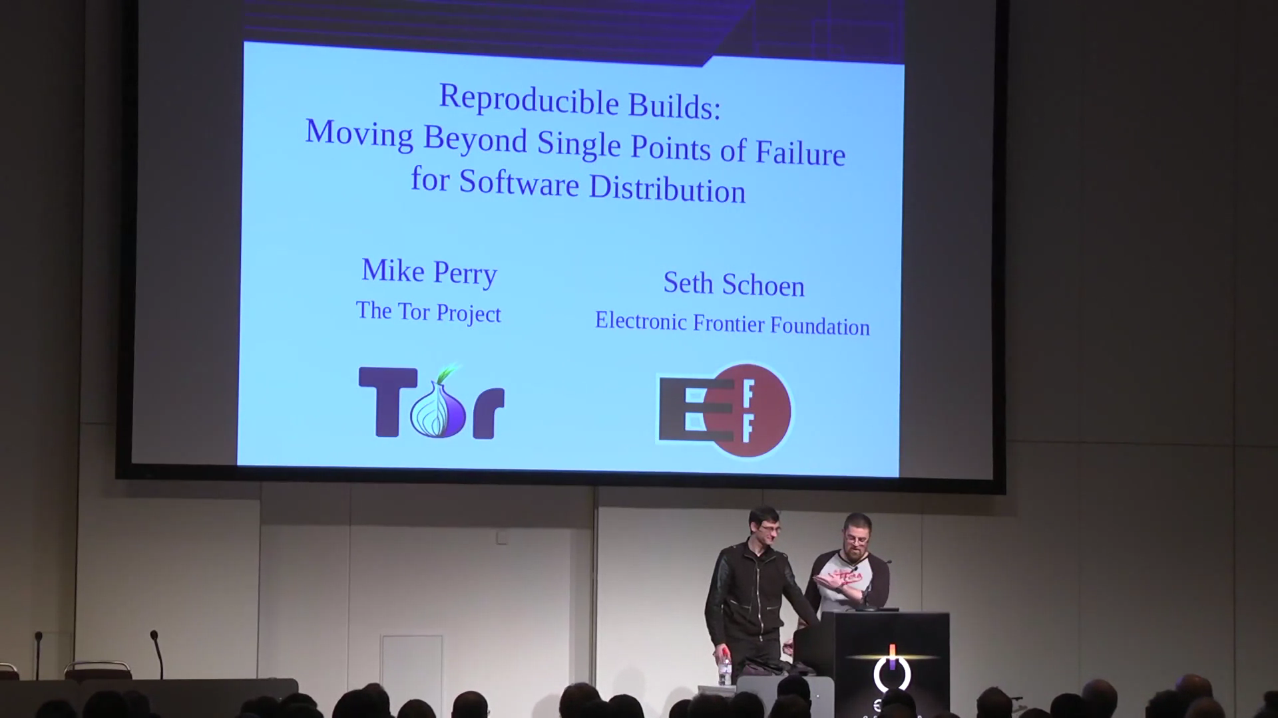
\includegraphics[width=0.7\textwidth]{images/31c3.png}

  Available on \url{media.ccc.de}, 31c3
 \end{center}
\end{frame}

\begin{frame}[fragile]
 \frametitle{A few examples from that 31c3 talk}
 \begin{itemize}
  \item CVE-2002-0083: remote root exploit in \texttt{sshd}, a single bit difference in the binary
  \item<2-5> 31c3 talk had a live demo with a kernel module modifying source code in memory only
  \item<3-5> How can you be sure what's running on your machine or on a build
  daemon network connected to the net? Do you ever leave your computers
  physically alone? 
  \item<4-5> How much do you pay your admins? Enough to withstand a multi million
  dollar attack?
  \item<5> Legal challanges. Could you be forced to backdoor (some of) your
  software (for some customers)?
 \end{itemize}
\end{frame}

\begin{frame}[fragile]
 \frametitle{Another example from real life}

 At a CIA conference in 2012:
 \begin{center}
  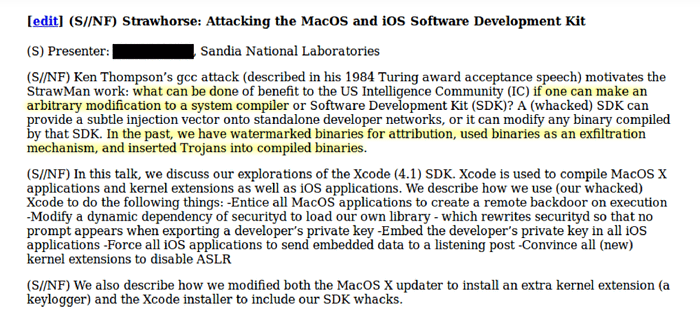
\includegraphics[width=0.8\textwidth]{images/strawhorse.png}

  {\footnotesize
  \url{firstlook.org/theintercept/2015/03/10/ispy-cia-campaign-steal-apples-secrets/}
  }
 \end{center}
\end{frame}


\begin{frame}
 \frametitle{The solution}

 \begin{center}
 \Large{
 Promise that anyone can always and independently generate
 identical binary packages from a given source}
\end{center}
\end{frame}


\begin{frame}
 \frametitle{The solution}

 \begin{center}
 We call this:

 \Huge{ “Reproducible builds” }
 \end{center}
\end{frame}

\placelogotrue

\begin{frame}
 \frametitle{Debian demo (skipped)}
 \begin{itemize}
 \item Build a package 5 times, get 5 .debs with different checksums
 \item Build a package 5 times, get 5 .debs with the same checksum\\
 \item<2-4>{Yes, it's really this simple.}
 \item<3-4>{And works the same with RPMs.}
 \item<4>{Signed RPMs are a bit more complicated but the principle stays the
same.}
 \end{itemize}
% show this once running in plain sid,
% and then in sid with our modified toolchain.
%
% prepare demo:
% mkdir demo ; cd demo ; apt-get source giftrans
%
% do demo:
% PTH=$(mktemp -d); OPTH=$PWD; P=giftrans; cp ${P}_* $PTH/; cd $PTH ;
%   dpkg-source -x ${P}*.dsc ; for X in 1 2 3 4 5 ; do (cd ${P}-*/;
%   dpkg-buildpackage -b -uc -us); mkdir -p .$X ; cp $P_*.deb .$X; done ; rm
%   *.deb ; echo; sha1sum *dsc *z .*/*.deb | grep -v giftrans-dbgsym ; cd - ;
% rm -r $PTH
\end{frame}

\placelogofalse

\begin{frame}[plain]
\begin{center}
 \Huge{This should become the \textbf{norm}.}

 \visible<2>{\small{ We want to change the meaning of "free software":

  it's only free software if it's reproducible!}}
\end{center}
\end{frame}

\begin{frame}[fragile]
 \frametitle{An important link in the chain of secure software distribution}
 \begin{itemize}
  \item But it's just one link in a big chain.
  \item Software security consists of more than secure distribution. I won't go into detail here, but think software lifecycle management.
  \item<2> It's a critical link though, linking sources to binaries and vice versa. The problem with randomness is, that one can never be sure. The problem with reproducible builds is, that it's a lot of efford to prove something, which we used to believe and take for granted.
  \item<2> Reproducible Builds are just one link in a big chain, turning that chain into a foundation to build trust upon. There are many ways to subvert this trust, but that's no excuse to stay a believer.
 \end{itemize}
\end{frame}


\begin{frame}[fragile]
 \frametitle{More benefits than "just" security…}
 \begin{itemize}
  \item Lots and lots of QA benefits - we've found so many subtile bugs.
  \item<2-5> Google does reproducible builds, to save time and money.
  \item<3-5> Smaller deltas, thus faster updates possible (for packages and
  images).
  \item<4-5> Side effect: meaningful binary diff between two versions.
  \item<5> …
 \end{itemize}
\end{frame}


\begin{frame}
 \frametitle{Some milestones in history}
 \begin{itemize}
\item<7> Cygnus.com (1992)
\item Bitcoin (2011)
\item<2-7> Tor (2013)
\item<3-7> Debian (2013, but really in 2014, and 2017 in \texttt{debian-policy})
\item<4-7> Core Infrastructure Iniative (2014)
\item<5-7> FreeBSD, coreboot, LEDE, openSUSE, NetBSD (2016++)
\item<6-7> Tails (2017)
 \end{itemize}
\end{frame}

\placelogotrue

\begin{frame}
 \frametitle{2017: Stretch at 94\% and in \texttt{debian-policy}}
 \begin{tikzpicture}[remember picture]
  \node[shift={(-0.5\paperwidth, \paperheight)},at=(current page.south east)] {
    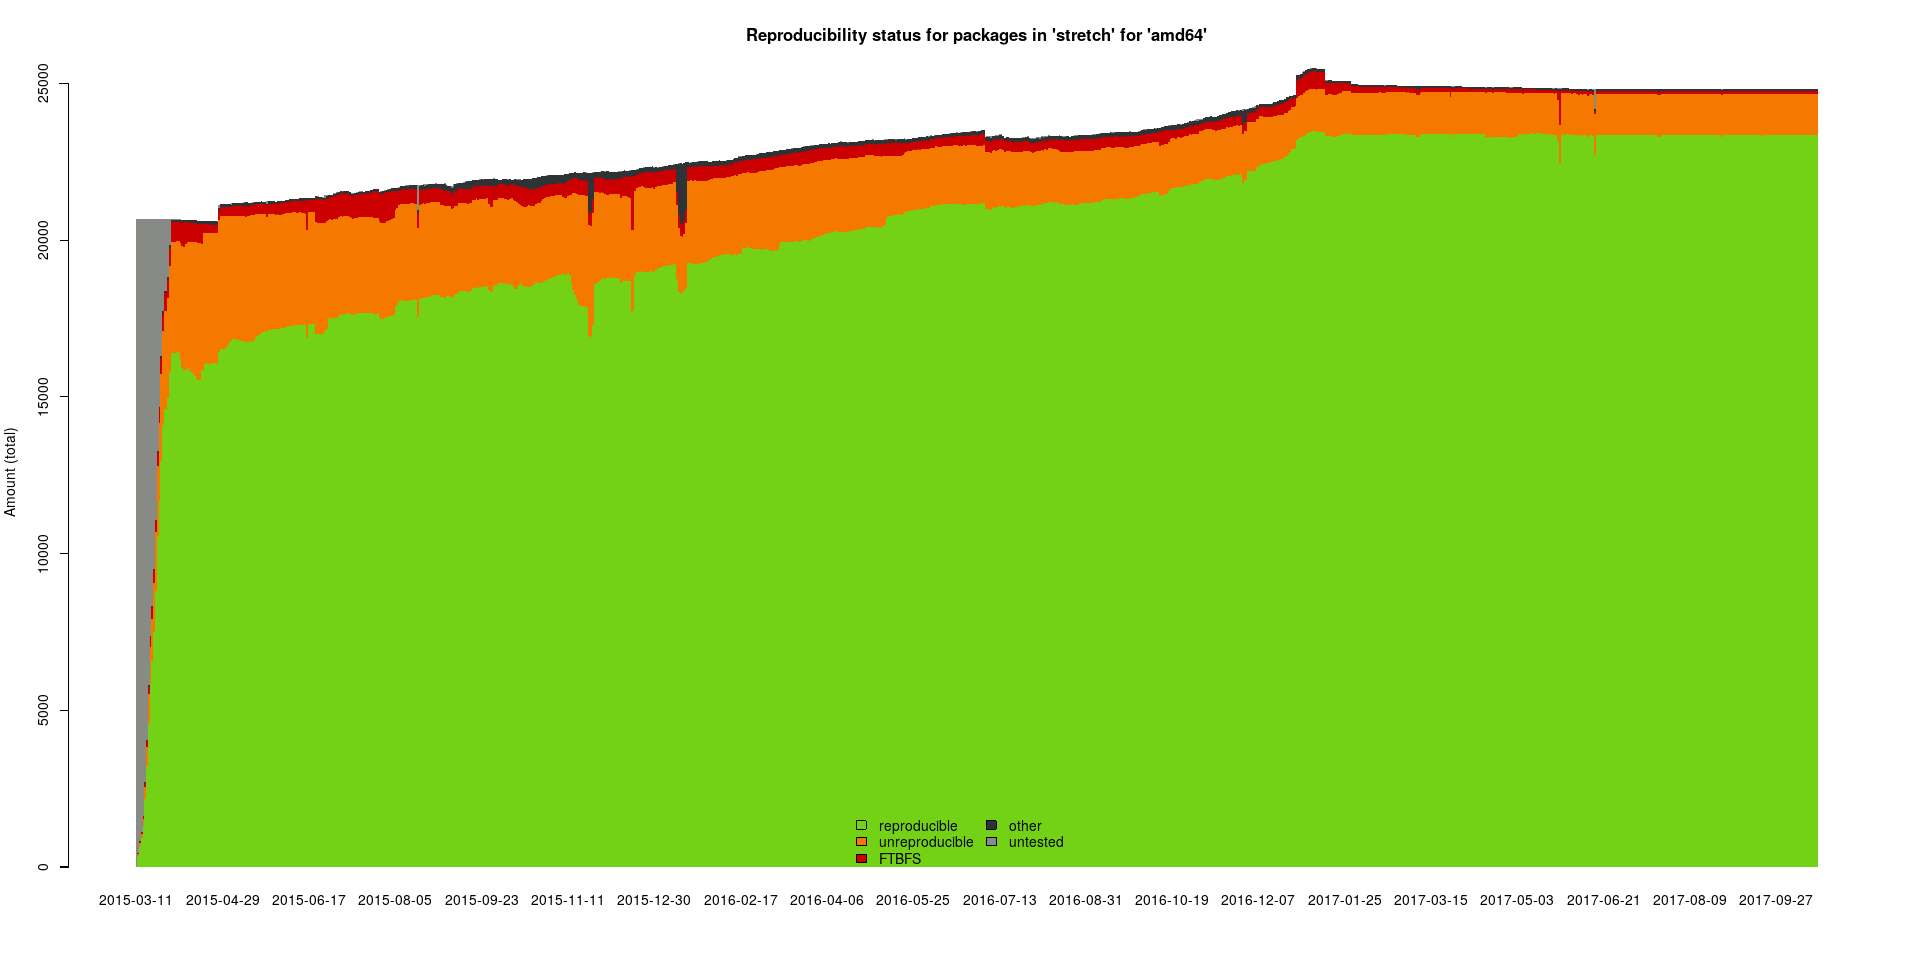
\includegraphics[height=0.65\paperheight]{images/stats_pkg_state_testing.png}
  };
 \end{tikzpicture}
 \begin{center}
  \footnotesize{23,344 (94.0\%) out of 24,821 source packages are reproducible \\
    in our test framework on \texttt{amd64}}
  \vfill
 \end{center}
\end{frame}

\placelogotrue

\begin{frame}
 \frametitle{"Misleading success"}
 \begin{itemize}
	 \item<2-4> In Debian in 2017 Reproducible Builds went into \texttt{debian-policy} and hopefully by 2019 we'll have \textbf{some} infrastructure and \textbf{some} user tools. But definitly we will not have reached 100\% Reproducible Builds before 2021, hopefully by then. 6\% is a lot if you're talking about 25000 packages but people seem to forget this.
	 \item<3-4> Despite the Debian developer community strongly supporting this, progress is difficult: it really get's complicated again on the last miles. (Think: 6\%, infrastructure \& user tools.)
	 \item<4> I might be wrong, I hope I am, but I only know of two other ("big or relevant", sorry) projects with similar commitment: Tails and Tor. But for them, a small How-To is sufficient.
 \end{itemize}
\end{frame}

\begin{frame}
 \frametitle{"Misleading success, cont."}
 \begin{itemize}
 \item Let me try to explain the problem: we are at 94\% of \textbf{theoretically} being able to do Reproducible Builds. Which means: the software supports it, in theory! What's lacking is infrastructure (think distribution of all those hashes) and user tools, so users can benefit from it.
 \item<2-4> Debian is the most advanced (big distro) here. The others haven't even started.
 \item<3-4> We need to keep doing what we have been doing (and which I'm going to explain in more detail) and we need to do more and new things. And we need \textbf{you} to join this efford, especially if you are not using Debian!
 \item<4> First 90\% take 90\% of the time \& last 9\% take another 90\%…

 \end{itemize}
\end{frame}

\section{Common ressources}

\begin{frame}
 \frametitle{reproducible-builds.org}

 \begin{itemize}
  \item \texttt{https://reproducible-builds.org}
  \item git repositories, IRC channels, mailinglists, webspace
 \end{itemize}
 \begin{center}
 
\includegraphics[width=0.7\textwidth]{images/rbwww1.png}
 \end{center}
\end{frame}


{
\usebackgroundtemplate{%
 \begin{tikzpicture}[remember picture,overlay]%
  \node[shift={(-0.1\paperwidth, 0.15\paperheight)},at=(current page.south east)] {
    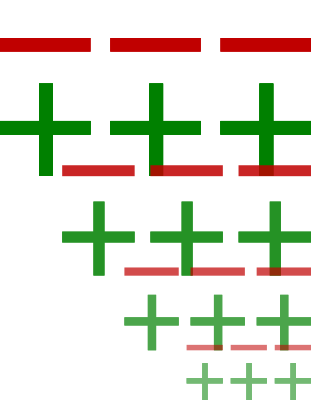
\includegraphics[width=0.2\paperwidth]{images/diffoscope_logo.png}
  };
 \end{tikzpicture}%
}

\begin{frame}{diffoscope}
 \frametitle{Debugging problems: \texttt{https://try.diffoscope.org}}

 \begin{itemize}
  \item Examines differences \textbf{in depth}.
  \item Recursively unpacks archives, uncompresses PDFs, disassembles
  binaries, unpacks Gettext files, …
  \item Easy to extend to new file formats.
  \item Falls back to binary comparison.
  \item Outputs HTML or plain text with human readable differences.
  \item Available from \texttt{git}, PyPI, Debian, \\
   Arch Linux, Guix, Homebrew, Fedora. Works on BSD.
  \item Maintainers in other distros wanted.
  \item \url{https://diffoscope.org/}
 \end{itemize}
\end{frame}


\begin{frame}
 \frametitle{\texttt{diffoscope} example (HTML output)}
 \begin{tikzpicture}[remember picture]
  \node[at=(current page.center)] {
   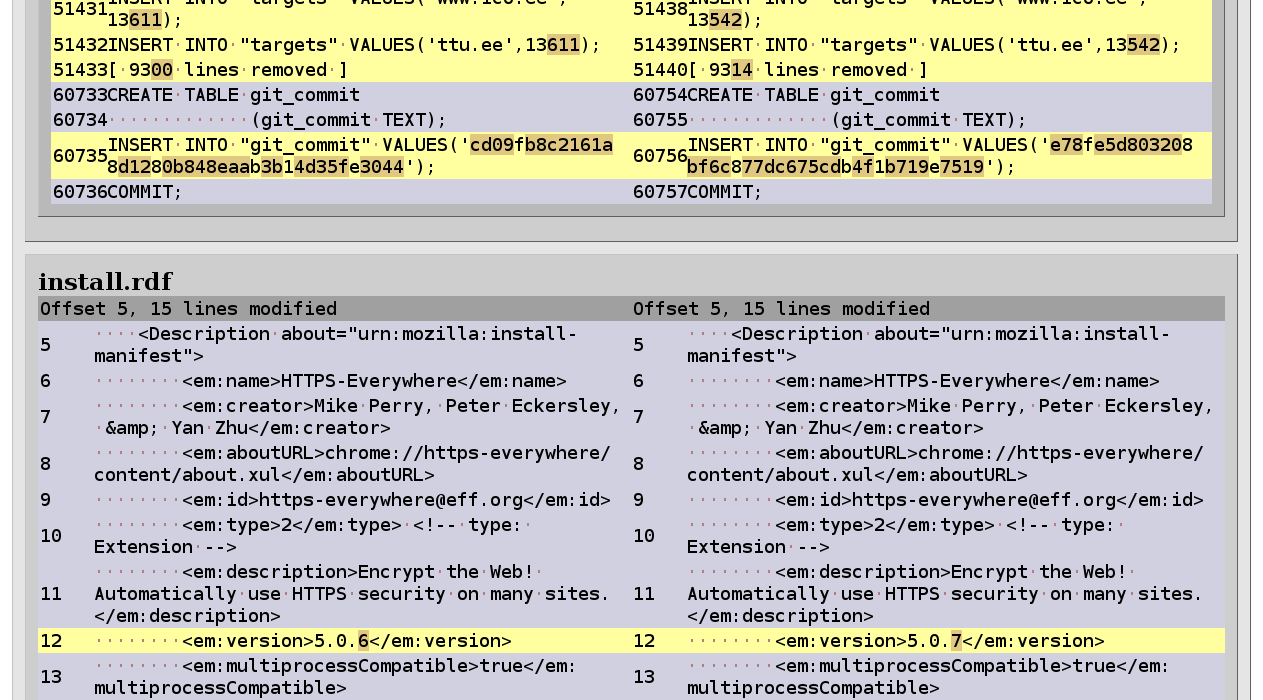
\includegraphics[width=0.9\paperwidth]{images/diffoscope_example_html.png}
  };
 \end{tikzpicture}
\end{frame}


\begin{frame}
 \frametitle{\texttt{diffoscope} is "just" for debugging}

 \begin{itemize}
  \item Reminder: \texttt{diffoscope} is for \textbf{debugging}
  \item "reproducible" according to our definition means: \textbf{bit by bit
  identical}. So the tools for testing whether something is reproducible are
  either \texttt{diff} or \texttt{sha256sum}!
  \item<2> \texttt{https://try.diffoscope.org}
 \end{itemize}
\end{frame}

}



\placelogofalse


\begin{frame}
 \frametitle{tests.reproducible-builds.org}

 \begin{itemize}
  \item Continuously testing Debian \texttt{testing}, \texttt{unstable} and
  \texttt{experimental} 
  \item Also testing: coreboot, LEDE, NetBSD, FreeBSD and F-Droid.
  Unmaintained tests: Arch Linux, Fedora and OpenWrt.
  \item 51 nodes (amd64/i386/arm64/armhf), 500 cores and 1 TB RAM
  \item 513 jenkins jobs running on jenkins.debian.net
  \item 51 scripts in Python and Bash, 357 lines of code in average
  \item 39 contributors for \texttt{jenkins.debian.net.git}
 \end{itemize}
 \begin{center}
  
\includegraphics[height=0.1\paperheight]{images/profitbricks_logo.png}
  \hspace{0.1\paperwidth}
  
\includegraphics[height=0.1\paperheight]{images/profitbricks_logo.png}
  \hspace{0.1\paperwidth}
  
\includegraphics[height=0.1\paperheight]{images/codethink.png}
  \hspace{0.1\paperwidth}
 
\includegraphics[height=0.1\paperheight]{images/debian_logo.png}
  \hspace{0.1\paperwidth}
 \end{center}
\end{frame}

\placelogotrue

\begin{frame}[fragile]
 \frametitle{Variations (when testing Debian)}

 \begin{center}
  \begin{table}
   \resizebox{0.95\textwidth}{!}{%
    \begin{tabular}{l|ll}
\textbf{variation} & \textbf{first build} & \textbf{second build} \\
\hline
hostname & \texttt{jenkins} & \texttt{i-capture-the-hostname} \\
domainname & \texttt{debian.net} & \texttt{i-capture-the-domainname} \\
\texttt{env TZ} & \texttt{GMT+12} & \texttt{GMT-14} \\
\texttt{env LANG} & \texttt{C} & \texttt{fr\_CH.UTF-8} \\
\texttt{env LC\_ALL} & not set & \texttt{fr\_CH.UTF-8} \\
\texttt{env USER} & \texttt{pbuilder1} & \texttt{pbuilder2} \\
uid & \texttt{1111} & \texttt{2222} \\
gid & \texttt{1111} & \texttt{2222} \\
UTS namespace & shared with the host & \textit{modified using \texttt{/usr/bin/unshare --uts}} \\
kernel version & Linux 3.16 or 4.X & on amd64 always varied, on armhf
sometimes \\
umask & 0022 & 0002 \\
CPU type & \multicolumn{2}{l}{varied on i386} \\
 & on armhf varied a bit, not on amd64 & \\
filesystem & \multicolumn{2}{l}{same for both builds on amd64: (\texttt{tmpfs}), on armhf \texttt{ext3/4}} \\
 & & \textit{(and we have} \texttt{disorderfs}\textit{, but the code is disabled)} \\
year, month, date & \multicolumn{2}{l}{on amd64: 398 days variation, on armhf not yet} \\
hour, minute & \multicolumn{2}{l}{hour is usually the same… usually, the minute differs… } \\
\textit{everything else} & \multicolumn{2}{l}{\textit{is likely the same…}}
    \end{tabular}
   }
  \end{table}
 \end{center}
\end{frame}

\placelogofalse

\begin{frame}
 \frametitle{Common problems}

 \begin{itemize}
  \item time stamps
  \item timezones
  \item locales
  \item build paths
  \item everything else (seperated into known issues and the blurry rest)
 \end{itemize}
\end{frame}

\begin{frame}
 \frametitle{Documentation about common problems}
 \begin{itemize}
  \item \texttt{https://reproducible-builds.org/docs}
  \item Lunar's talk from CCCamp 2015 also on
  \texttt{https://media.ccc.de}
 \begin{tikzpicture}[remember picture]
  \node[shift={(-1.05\paperwidth, -0.3\paperheight)},at=(current page.south east)] {
    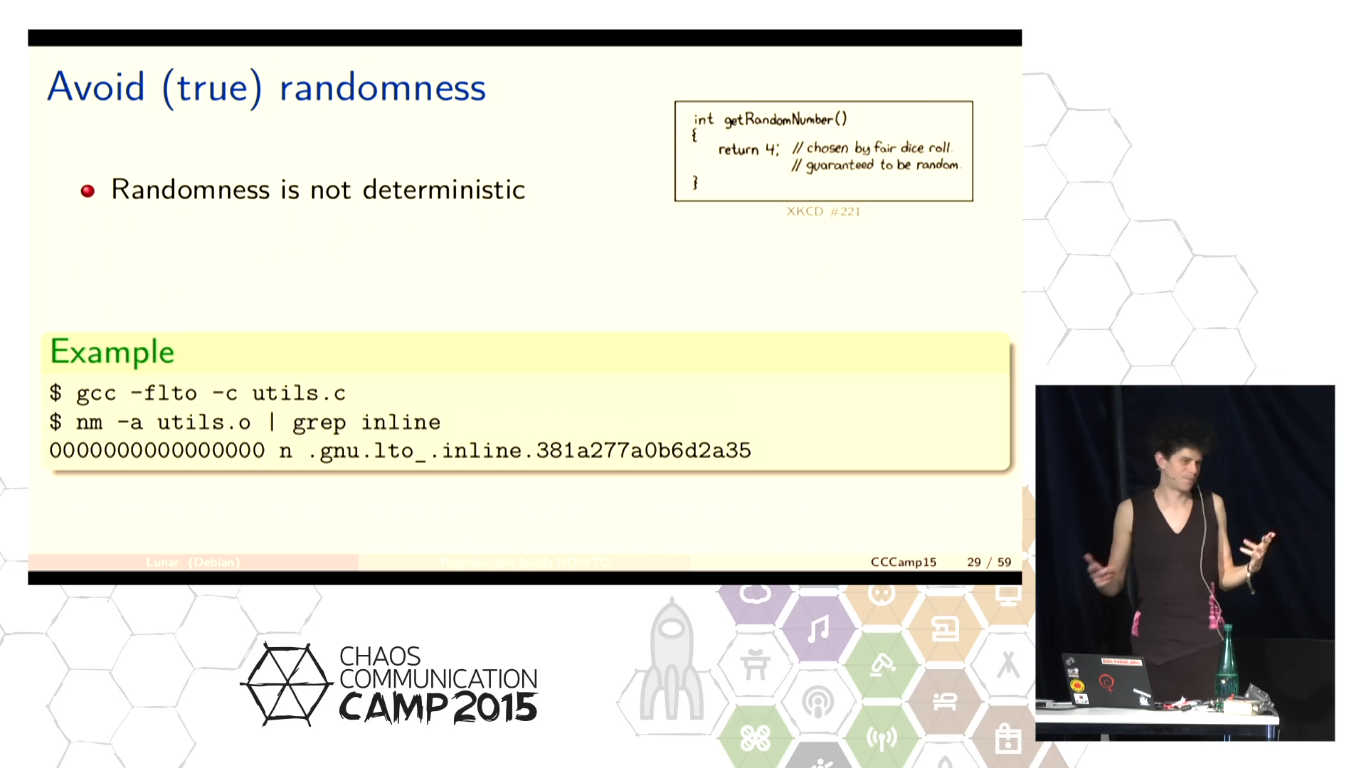
\includegraphics[width=0.83\textwidth]{images/cccamp2015_lunar_random.png}
  };
 \end{tikzpicture}
 \end{itemize}
\end{frame}


\begin{frame}
 \frametitle{\texttt{SOURCE\_DATE\_EPOCH}}

 \begin{itemize}
  \item Build date (timestamps) usually not useful for the user
  \item \texttt{SOURCE\_DATE\_EPOCH} is defined as the last modification of
  the source, since the epoch (1970-01-01)
  \item can be used instead of current date
  \item can also be used for random seeds etc.
  \item in Debian, set from the latest \texttt{debian/changelog} entry
  \item can be set to the latest git commit too or the latest file
  modification date
 \end{itemize}
\end{frame}

\begin{frame}
 \frametitle{\texttt{SOURCE\_DATE\_EPOCH}}

 \begin{itemize}
  \item \texttt{SOURCE\_DATE\_EPOCH} spec available:
  \item \texttt{https://reproducible-builds.org/specs/}
  \item many upstreams support it already
  \item has been adopted by other distributions
  (openSUSE, OpenWrt, LEDE, NetBSD, FreeBSD, Arch Linux, coreboot, Guix, …) and many many
  upstreams (GCC, dpkg, rpm, mkisofs, ghostscript, libxslt, sphinx,
  texlive-bin, …)
 \end{itemize}
\end{frame}

\begin{frame}
 \frametitle{two more tools}

 \begin{itemize}
  \item \texttt{strip-nondeterminism} 
  \item<2> \texttt{reprotest} 
 \end{itemize}
\end{frame}

\section{Status Debian}

\begin{frame}
 \frametitle{Status golang}

 \begin{itemize}
  \item<2-4> Golang binaries are bit by bit reproducible!
  \item<3-4> Except when the build path is varied…
  \item<4> \url{https://anonscm.debian.org/cgit/pkg-golang/golang.git/tree/debian/patches/0002-reproducible-BUILD\_PATH\_PREFIX\_MAP.patch?h=golang-1.9}

 \end{itemize}
 \begin{center}
  
\includegraphics[height=0.2\paperheight]{images/golang.png}
 \end{center}
\end{frame}

\begin{frame}
 \frametitle{\texttt{BUILD\_PATH\_PREFIX\_MAP}}
 \begin{itemize}
  \item "This specification describes the environment variable BUILD\_PATH\_PREFIX\_MAP for build tools to exchange information about the build-time filesystem layout, to generate reproducible output where all embedded paths are independent of that layout."
  \item \url{https://reproducible-builds.org/specs/build-path-prefix-map/}
  \item<2-3> Build path variations only enabled when testing Debian \texttt{unstable}.
  \item<3> The easy workaround today is to rebuild in the same path. But it is a workaround, why should the path be embedded in the binary?
 \end{itemize}
\end{frame}


\placelogotrue



\begin{frame}
 \frametitle{Progress in Debian \texttt{unstable}}
 \begin{tikzpicture}[remember picture]
  \node[shift={(-0.5\paperwidth, \paperheight)},at=(current page.south east)] {
    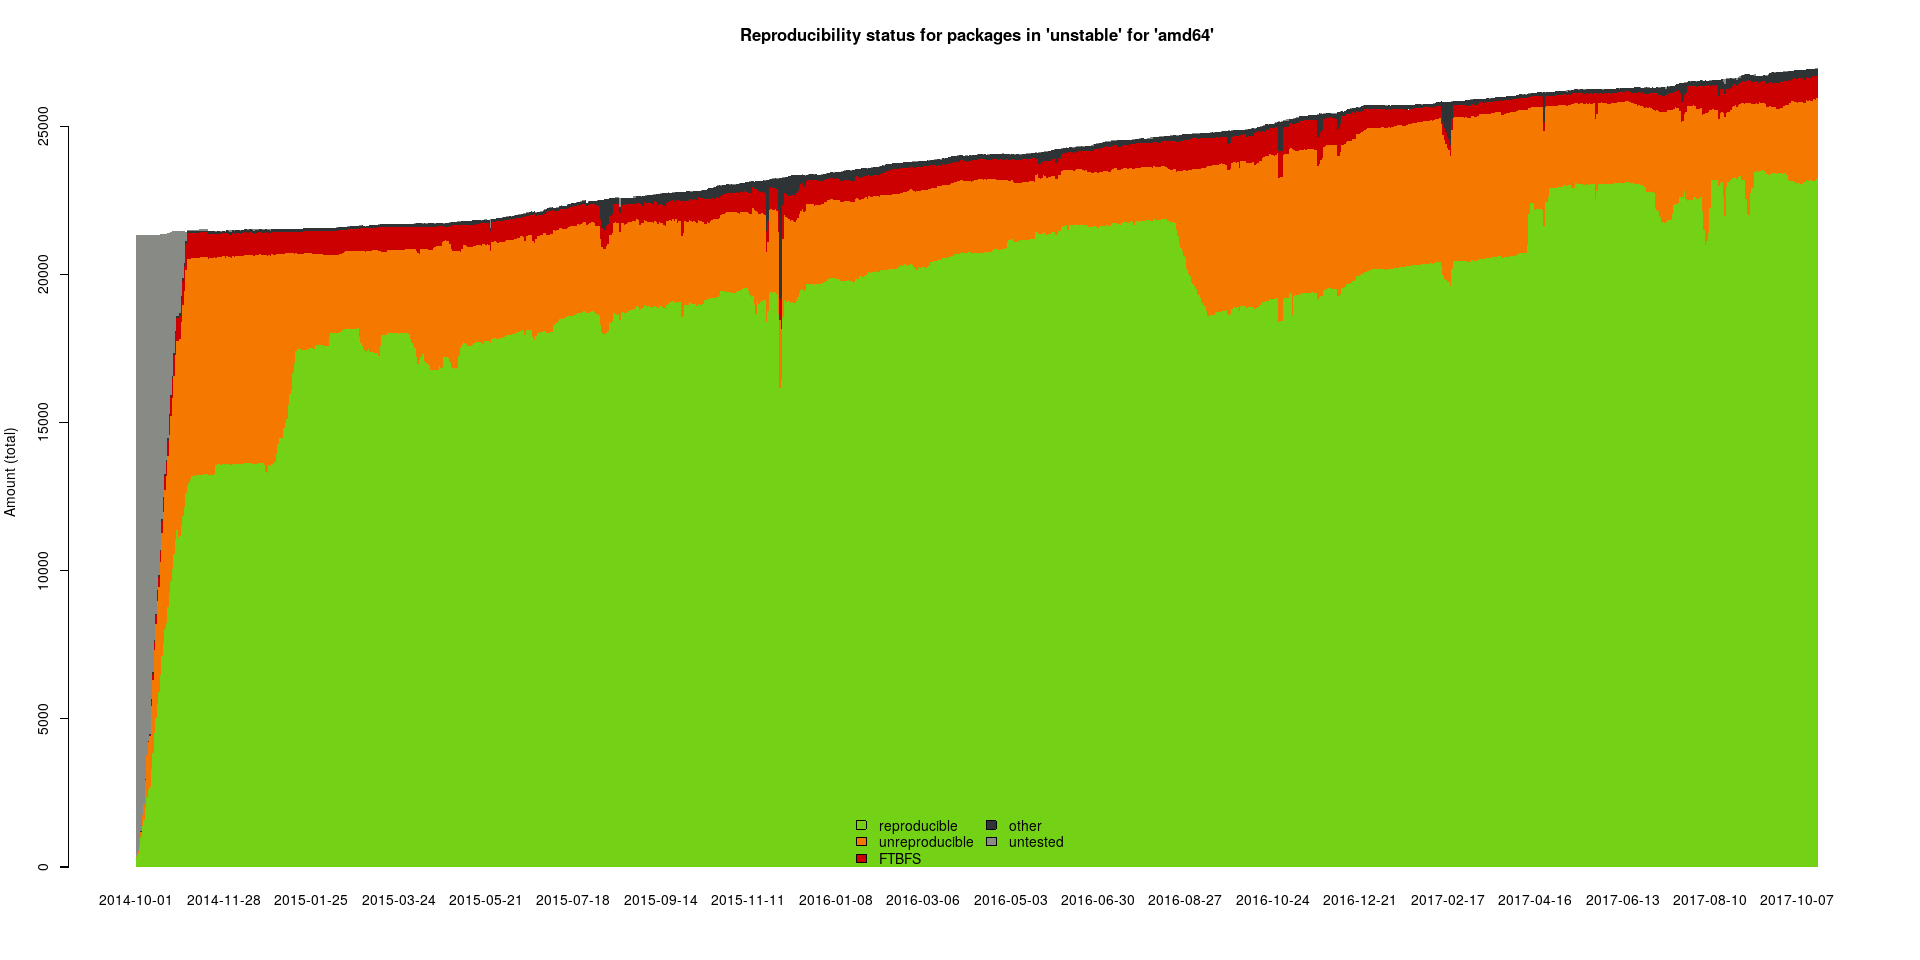
\includegraphics[height=0.65\paperheight]{images/stats_pkg_state_unstable.png}
  };
 \end{tikzpicture}
 \begin{center}
  \footnotesize{23,243 (86.2\%) out of 26,957 source packages are reproducible \\
    in our test framework on \texttt{amd64}} (difference due to build path variations)
  \vfill
 \end{center}
\end{frame}

\begin{frame}
 \frametitle{some more details on tests.reproducible-builds.org}

 \begin{itemize}
  \item \url{https://reproducible.debian.net/$src}
  \item<2> 49 package sets 
 \end{itemize}
\end{frame}

\begin{frame}
	\frametitle{Debian notes \& issues on tests.reproducible-builds.org}

 \begin{itemize}
  \item 283 categorised distinct issues
  \item 6,220 notes
  \item 1,594 unreproducible packages in \texttt{buster/amd64} (testing), but only
  263 without a note (3,433 in \texttt{unstable} but also only 378 without a
  note)
  \item maintained in \texttt{notes.git} by 58 contributors
  \item currently Debian only, but cross distro notes are planned
 \end{itemize}
\end{frame}


\begin{frame}
 \frametitle{Debian \texttt{.buildinfo} files}

 \begin{itemize}
  \item Aggregates in the same file:
   \begin{itemize}
    \item Sources (checksums)
    \item Generated binaries (checksums)
    \item Packages used to build (with specific version, checksums coming soon)
   \end{itemize}
  \item Can be later used to exactly recreate environment
  \item For Debian, all versions are available from \url{snapshot.debian.org}
 \end{itemize}
\end{frame}


\begin{frame}
 \frametitle{Progress in the Debian bug tracker}
 \begin{tikzpicture}[remember picture]
  \node[shift={(-0.5\paperwidth, \paperheight)},at=(current page.south east)] {
    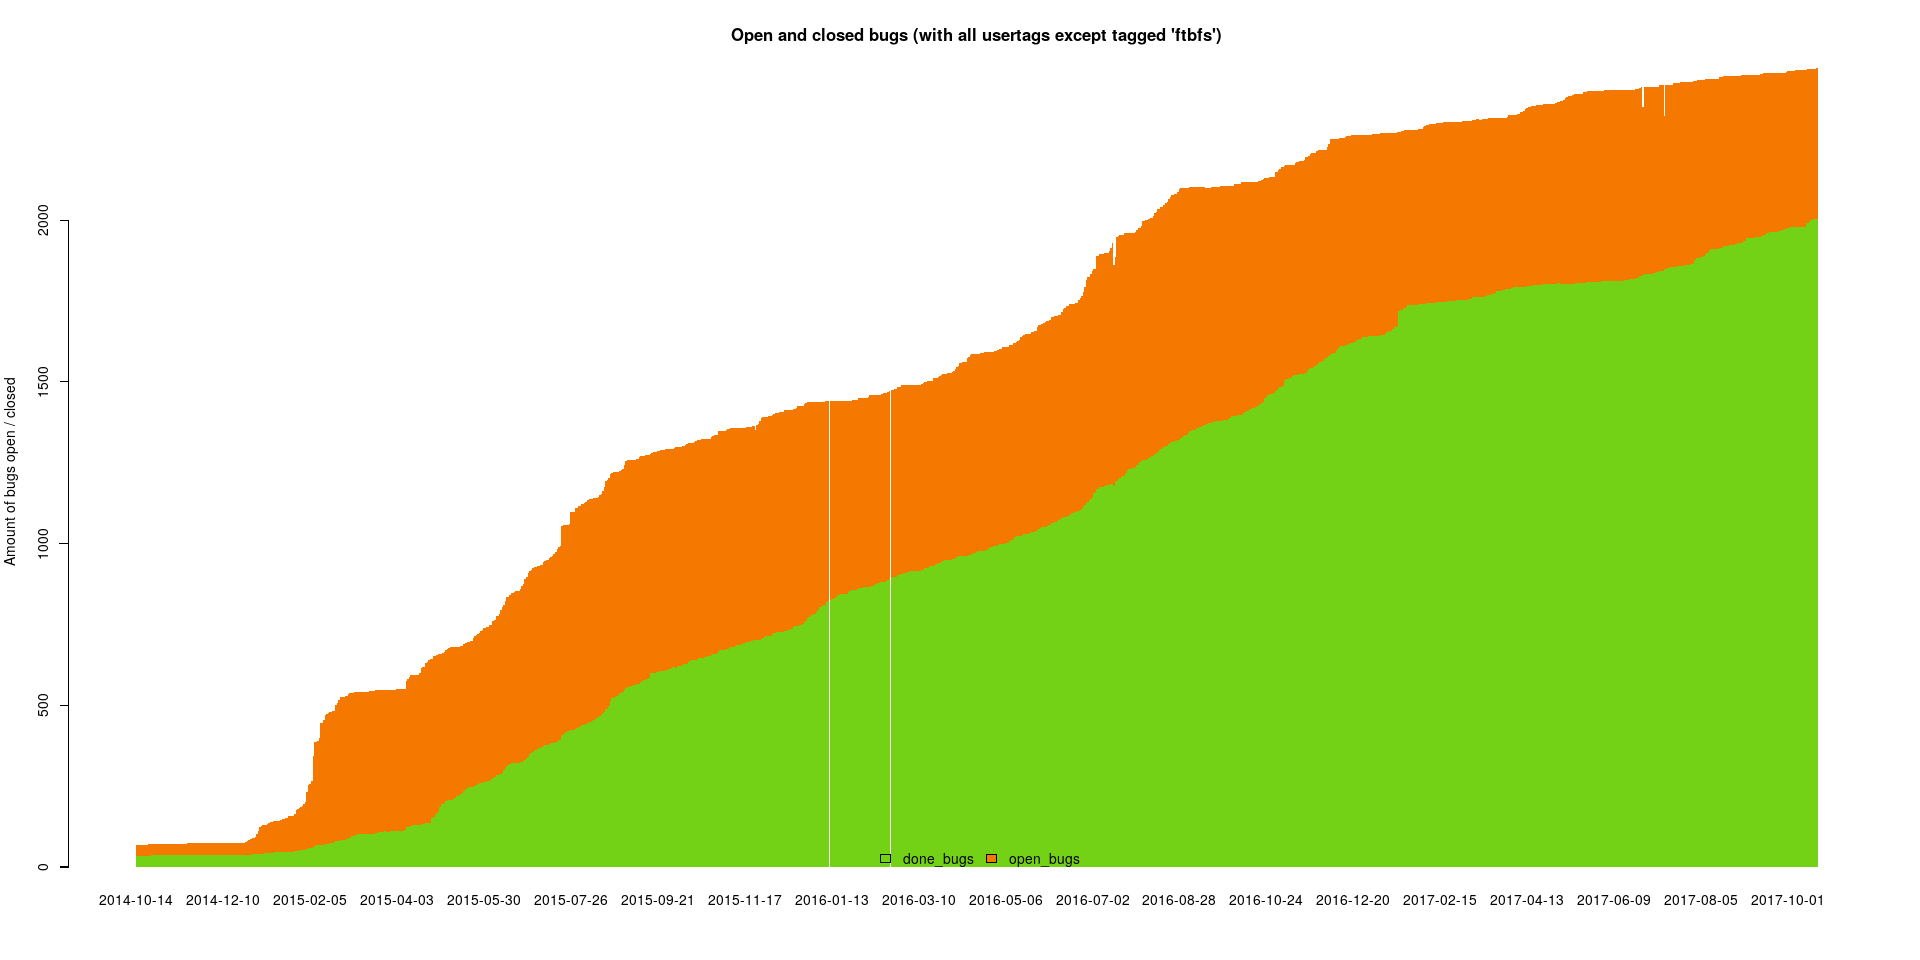
\includegraphics[height=0.65\paperheight]{images/stats_bugs_sin_ftbfs_state.png}
  };
 \end{tikzpicture}
 \begin{center}
  \footnotesize{As a rule, we file bugs with patches. \\
  There are very few exceptions.}
  \vfill
 \end{center}
\end{frame}



\begin{frame}
	\frametitle{Debian summary - situation in Stretch (Debian 9)}
 \begin{itemize}
  \item This is/was a proof-of-concept, Debian is neither 94\% reproducible nor
  86\%. (and 10\% > 2,500 sources packages!)
  \item<2-4> All our required changes have been included in Stretch!
  \item<3-4> 94\% of the source packages in Stretch can build reproducible packages. But less than 20\% of the released binaries are reproducible…
  \item<3-4> Because, Debian does not (yet?) do full rebuilds before
  releasing… so stuff is in the archive which is not reproducible unless it's
  rebuild.
  \item<4> And then we don't distribute \texttt{.buildinfo} files yet.
   That (and user tools) still needs more \it{design} and code.
 \end{itemize}
\end{frame}


\begin{frame}
	\frametitle{Debian summary - situation for derivates \& the future}
 \begin{itemize}
  \item Stretch's source code is 94\% reproducible and all required change are included.
  \item So others, eg Canonical can take our work now and make Ubuntu 17.10
  (partly) reproducible…
  \item<2-4> Debian 10, "buster", will be partly reproducible in 2019.
  \item<3-4> Since August 2017 \texttt{debian-policy} mandates that packages \textbf{should} be reproducible.
  \item<4> We hope \texttt{debian-policy} will mandate 100\%
	  reproducible builds ("\textbf{must}") for Debian 11, "bullseye", in 2021. And even then, there can be exceptions…
 \end{itemize}
\end{frame}

\begin{frame}
 \frametitle{Tell the world \& collaborate}

 \begin{itemize}
  \item "We don't care about Debian (only), we care about free and open
	  source software." (By now this is pretty obvious.)
  \item<2-4> 130 Weekly reports since May 2015
  \item<3-4> First Reproducible World Summit in December 2015 (Athens, Greece)
   \begin{itemize}
    \item<3-4> \texttt{reproducible.debian.net} has become \texttt{tests.reproducible-builds.org}
   \end{itemize}
    \item<3-4> Second Reproducible World Summit in December 2016 in Berlin
    \item<3-4> Third Reproducible World Summit at the End of October 2017 in Berlin - contact me if you want to attend.
   \item<4> GSoC and Outreachy
 \end{itemize}
\end{frame}



\section{Status Non-Debian World}

\placelogofalse

\begin{frame}
 \frametitle{Skipping some…}
 \begin{itemize}
  \item \texttt{https://tests.r-b.org/coreboot}
  \item \texttt{https://tests.r-b.org/netbsd}
  \item \texttt{https://tests.r-b.org/freebsd}
  \item paused: \texttt{https://tests.r-b.org/archlinux}
  \item almost there: \texttt{https://tests.r-b.org/f-droid}
  \item paused: {https://tests.r-b.org/openwrt}
  \item \texttt{https://tests.r-b.org/lede}
 \end{itemize}
 \begin{center}
  
\includegraphics[height=0.13\paperheight]{images/coreboot.png}
  \hspace{0.05\paperwidth}
  
\includegraphics[height=0.13\paperheight]{images/netbsd.png}
  \hspace{0.05\paperwidth}
  
\includegraphics[height=0.13\paperheight]{images/freebsd.png}
  \hspace{0.05\paperwidth}
  
\includegraphics[height=0.13\paperheight]{images/f-droid.png}
  \hspace{0.05\paperwidth}
  
\includegraphics[height=0.13\paperheight]{images/archlinux.png}
  \hspace{0.05\paperwidth}
  
\includegraphics[height=0.3\paperheight]{images/openwrt.png}
  \hspace{0.05\paperwidth}
  
\includegraphics[height=0.15\paperheight]{images/lede.png}
\end{center}
\end{frame}


\begin{frame}
 \frametitle{Skipping some more…}
 \begin{itemize}
\item Cygnus.com (1992)
\item Bitcoin (2011)
\item Tor (2013)
\item NixOS, GNU Guix, ElectroBSD
\item openSUSE
\item Qubes, Tails, webconverger
\item Google Bazil
\item ducible (build tool for Windows)
\item very few commercial, propietary software
 \end{itemize}
\end{frame}


\begin{frame}
 \frametitle{Detour: what, reproducible commercial Software???}
 \begin{itemize}
\item Guess which
\item <2-3>   windows? (the source is available)
\item <2-3>   medical devices in your body?
\item <2-3>   arms?
\item <2-3>   critical infrastructure like in nuclear powerplants?
\item <2-3>   cars?
\item <3> Gambling machines!
 \end{itemize}
\end{frame}


\section{Status RPM world: Fedora and openSUSE}

\begin{frame}
 \frametitle{reproducible openSUSE}
 \begin{itemize}
	 \item \url{https://en.opensuse.org/openSUSE:Reproducible\_Builds}
  \item Bernhard Wiedemann started this in 2016
  \begin{itemize}
   \item build-succeeded: 11594
   \item bit-by-bit-identical: 11111
   \item not-bit-by-bit-identical: 478
 \end{itemize}
  \begin{itemize}
   \item<2-4> 102 undeterministic from javadoc output
   \item<2-4> 22 undeterministic from latex
   \item<2-4> 12 undeterministic from mono
   \item<2-4> 20 undeterministic from Qt
 \end{itemize}
 \item<3-4> Results not included into \url{tests.r-b.o} yet.
 \item<4> Bernhard also deserves credit for creating \texttt{https://github.com/orgs/distropatches} and sending many patches upstream.
 \end{itemize}
 \begin{tikzpicture}[remember picture,overlay]
  \node[shift={(-0.1\paperwidth, 0.13\paperheight)},at=(current page.south east)] {
    
\includegraphics[height=0.15\paperheight]{images/openSUSE.png}
  };
 \end{tikzpicture}
\end{frame}


\begin{frame}
 \frametitle{What's going well in the rpmworld}
 \begin{itemize}
  \item \texttt{rpm} respects SOURCE\_DATE\_EPOCH.
  \item \texttt{yum} and \texttt{dnf} might create non-identical environments
  \item \texttt{diffoscope} is available in Fedora and openSUSE:
  \item signed RPMs -> re-apply signature, will match for identical builds
  \item<2> Bernhard.
  \end{itemize}
 \begin{center}
  
\includegraphics[height=0.1\paperheight]{images/openSUSE.png}
  \hspace{0.1\paperwidth}
 
\includegraphics[height=0.1\paperheight]{images/fedora.png}
  \hspace{0.1\paperwidth}
 \end{center}

\end{frame}


\begin{frame}
 \frametitle{Not going so well in the rpmworld yet}
 \begin{itemize}
	 \item Bernhard (and very few others)
  \end{itemize}
 \begin{center}
  
\includegraphics[height=0.1\paperheight]{images/openSUSE.png}
  \hspace{0.1\paperwidth}
 
\includegraphics[height=0.1\paperheight]{images/fedora.png}
  \hspace{0.1\paperwidth}
 \end{center}

\end{frame}

\begin{frame}
 \frametitle{Not going so well in the rpmworld…}
 \begin{itemize}
	 \item No wide / community commitment.
	 \item<2-3> no \texttt{.buildinfo} files, thus no tools to use them…
	 \item<2-3> no user tooling yet.	 
	\item<3> This is not limited to the rpmworld :/
  \end{itemize}
 \begin{center}
  
\includegraphics[height=0.1\paperheight]{images/openSUSE.png}
  \hspace{0.1\paperwidth}
 
\includegraphics[height=0.1\paperheight]{images/fedora.png}
  \hspace{0.1\paperwidth}
 \end{center}

\end{frame}





\section{Future work}

\begin{frame}
 \frametitle{Future work}
 \begin{itemize}
 \item<1-3> So far we mostly worked on making reproducible builds possible…
 \item<2-3> We'll need constant tests for future code.
 \item<3> And then, this still needs tools, infrastructure and policies to become
 meaningful and to be used in practice.
 \end{itemize}
\end{frame}

\begin{frame}
 \frametitle{Rebuilds and sharing signed checksums}
 \begin{itemize}
  \item Almost no work has been done here yet. We are just at the first step:
  being able to rebuild reproducibly…
  \item Different projects, different solutions?
 \begin{itemize}
  \item<2> something like \texttt{.buildinfo} files (defining the environment,
  the input and the output(s)) will be needed everywhere:
  \item<2> implemented for Debian (both in sbuild and well as
  buildinfo.debian.net)
  \item<2> work has begun for coreboot, LEDE/OpenWrt and Fedora (mock/koji)
  and maybe openSUSE (OpenBuildService)
 \end{itemize}
 \end{itemize}
\end{frame}

\begin{frame}
 \frametitle{Rebuilders and sharing signed checksums, cont.}
 \begin{itemize}
  \item Individuelly signed checksums (think web of trust) could work in the
  Debian case (we have a gpg web of trust), but IMO won't scale.
  \item { Another idea: rebuilders, run by large organisations
  (ACLU, CCC, Deutsche Bank, Greenpeace, NASA, NSA, US-Army).}
  \item Fedora rebuilds Debian, Debian rebuilds openSUSE, openSUSE rebuilds
  NetBSD, etc…
  \item Big customers could just rebuild everything themselves.
 \end{itemize}
\end{frame}


\begin{frame}
 \frametitle{Integration in user tools}
 \begin{itemize}
  \item "Do you really want to install this unreproducible software (y/N)"
  \item<2-3> "Do you want to build those packages which have unconfirmed checksums,
  before installing? (Y/n)"
  \item<3>{ "How many signed checksums do you require to call a package
  'reproducible'?" - and whom do you trust?}
 \end{itemize}
\end{frame}


\section{Getting involved}

\begin{frame}
 \frametitle{As a software developer}
 \begin{itemize}
  \item Stop using build dates
  \item Use \texttt{SOURCE\_DATE\_EPOCH} instead
  \item See \url{https://reproducible-builds.org/specs/}
  \item<2> Attend the summit in Berlin? (31 Oct. + 1+2 Nov)
 \end{itemize}
\end{frame}


\begin{frame}
 \frametitle{Form your reproducible builds team!}
 \begin{itemize}
  \item Why?
   \begin{itemize}
    \item Every distribution should be reproducible!
    \item Learn something new everyday
    \item Change the (software) world!
    \item \texttt{https://tests.reproducible-builds.org/XYZ} needs \textbf{your} help
   \end{itemize}
  \item How to get started?
   \begin{itemize}
    \item Build something twice, run diffoscope on the results.
    \item Experiment - learning by doing
    \item RTFM, there is lots of documentation
    \item Talk to us (or myself) on IRC or via mail.
   \end{itemize}
 \end{itemize}
\end{frame}

\section{Questions, comments, ideas?}

\placelogotrue

\begin{frame}
 \frametitle{Thanks to…! …and thank \textbf{you}, too!}

 \begin{itemize}
  \item
    {All “Reproducible Builds” contributors \\
        {\small (you are just \textbf{so} awesome!)}}
  \item All Systems Go!
\end{itemize}

 \begin{center}
  
\includegraphics[height=0.1\paperheight]{images/linux_foundation_logo.png}
  \hspace{0.1\paperwidth}
  
\includegraphics[height=0.1\paperheight]{images/cii_logo.png}
 \end{center}

 \vfill
 \begin{center}
  \resizebox{0.9\textwidth}{!}{%
   \begin{tabular}{rl}
    \texttt{holger@debian.org} & \texttt{B8BF 5413 7B09 D35C F026} \\
                               & \texttt{FE9D 091A B856 069A AA1C}
\end{tabular}
  }
 \end{center}
\end{frame}

\placelogofalse

\begin{frame}
 \frametitle{Questions, comments, ideas?}

 \begin{itemize}
  \item \url{https://reproducible-builds.org/}
  \item \texttt{\#reproducible-builds} on \texttt{irc.OFTC.net}
  \item \url{https://lists.reproducible-builds.org}
  \item twitter: @ReproBuild
  \item<2> Mike and Seth's talk from 31c3 about motivations
  \item<2> Lunar's talk about fixing reproducible issues from CCCamp 15
  \end{itemize}
\end{frame}

\placelogotrue

\begin{frame}{}
\begin{textblock}{12}(2, 6)
    \tiny{
      Copyright \copyright{} 2014--2017 \\
         Holger Levsen \texttt{holger@layer-acht.org} and others.\\[3.0mm]
      Copyright of images included in this document are held by
      their respective owners.
      \\[3.0mm]
      This work is licensed under the \alert{Creative Commons
        Attribution-Share Alike 3.0} License.  To view a copy of this
      license, visit
      \url{http://creativecommons.org/licenses/by-sa/3.0/} or send a
      letter to Creative Commons, 171 Second Street, Suite 300, San
      Francisco, California, 94105, USA.
      \\[2.0mm]
      % Give a link to the 'Transparent Copy', as per Section 3 of the GFDL.
      The source of this document is available from
      \url{https://anonscm.debian.org/git/reproducible/presentations.git}.
    }
  \end{textblock}
\end{frame}

\end{document}
